\section{Des indiens dans la ville}

1 fév. 2008

\begin{multicols}{2}


Aujourd'hui visite du centre de Delhi et plus spécialement le coin de Connaught Place, tout cela après un petit déjeuner indiano-européen sur le toit de l’hôtel, au 5ème étage, avec vue sur les environs. Une super rencontre au milieu du parc public de Connaught Place avec Raja et Showkat qui nous invitent à prendre un indian tea dans une petite boutique genre snack, nous passons deux heures à discuter avec eux, ils nous ont appris quelques mots d’Hindi qui vont nous être très utiles (on dit namasté pour dire bonjour ou au revoir, ça on le savait, ensuite pour dire merci c’est daniwad et je n’ai besoin de rien se dit chalo). Nous avons alors testé notre nouveau vocabulaire et c’est impressionnant de voire le changement de réaction des gens quand on leur dit un mot dans leur langue. Dire I dont need anything ne sert pas à grand chose alors que dire chalo nous donne droit à un sourire respectueux et aucune insistance de la part du vendeur.

\smallbreak
\hspace*{-0.65cm}
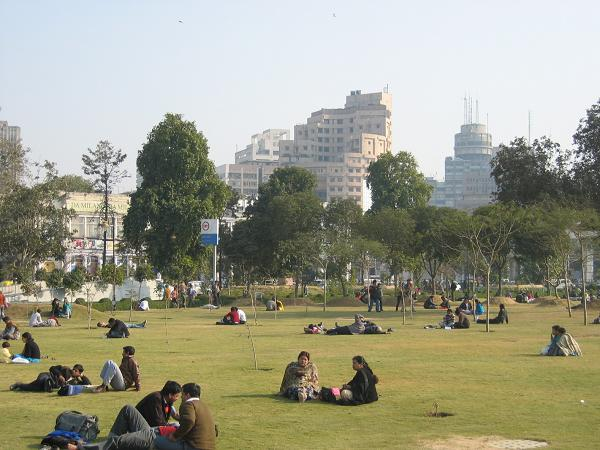
\includegraphics[width=5cm]{articles/Des-indiens-dans-la-ville/connaughtplace.jpg}
\smallbreak

%// TODO : Expliquer la méprise.

Après ça on a essayé de se renseigner sur les trains pour commencer notre tour.
Première boutique, clairement arnaqueuse et habituée aux touristes (d’ailleurs le prix est en euros), mais un chauffeur de rickshaw nous indique une meilleure adresse et il s’agit de la boutique recommandée par le Lonely Planet.

\smallbreak
\hspace*{-0.65cm}
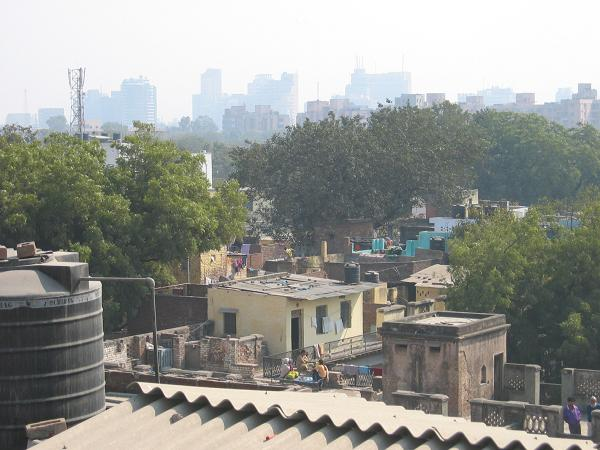
\includegraphics[width=5cm]{articles/Des-indiens-dans-la-ville/toithotel.jpg}
\smallbreak

Et là... c’est le drame... imaginez le Rajasthan grand comme à peu près deux tiers de la France, mettez y quelques lignes de trains reliant uniquement les grandes villes et une énorme population (12 millions d'habitants à New Delhi). Il faut donc réserver bien à l’avance son trajet, nous n’avons rien avant 12 jours.
On va donc prendre les billets correspondant à la deuxième partie de notre voyage demain et nous devrons nous passer de train pour la première partie (bus, rickshaw...).

\smallbreak
\hspace*{-0.65cm}
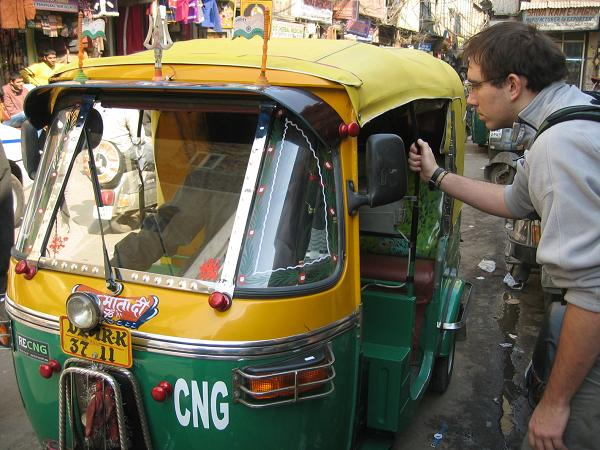
\includegraphics[width=5cm]{articles/Des-indiens-dans-la-ville/ricksaw.jpg}
\smallbreak

%// TODO : Expliquer l'arnaque.

En tout cas niveau repas c’est excellent, et piquant... le respect de l’hygiène est assez folklorique... mais on est pas là pour ça.

\end{multicols}

\pagebreak\bigskip
\textbf{\textsc{Commentaires}}

\medskip
Peggy a écrit le 1 fév. 2008 :
\begin{displayquote}
Ah une photo de d'Etienne, il est vivant!!
Vous êtes très très débrouillards..*impressionée*
Comment dit on "à bientôt" ??
\end{displayquote}

\medskip
Titou a écrit le 1 fév. 2008 :
\begin{displayquote}
Yeah je suis super content de voir que vous vous sentez déjà comme chez vous là bas ! La preuve vous avez déjà fait un troquet ! Bon ok, pour une fois c'était pour boire du thé\dots Mais quand même ! Eclatez vous et à bientôt !
\end{displayquote}

\medskip
Mam' a écrit le 2 fév. 2008 :
\begin{displayquote}
Bien sympa de recevoir un petit coup de fil d'Inde quand on est tout juste réveillée et encore au lit, du coup cela m'a permis de replonger sous la couette pour rêver de Taj-Mahal au lever du soleil, de Jophur(au fait vérifez si la forme des pantalons est bien ce que nous, nous appellons Jodphur!) et de citadelles, palais de maharadjas!!!. Je vous souhaite plein de rencontres. Buvez un lhassi à la santé des blogueurs "Didoum"de notre belle France. Bisou et à bientôt le plaisir de vous lire. Namaste.
\end{displayquote}

\medskip
Tatid a écrit le 21 fév. 2008 :
\begin{displayquote}
Les Indiens ont l'air vraiment accueillants, c'est sympa ça ! J'imagine que vous communiquez en anglais, ça doit être assez drôle un indien qui parle anglais, il doit falloir un temps d'adaptation\dots !
Namaste !
\end{displayquote}

\vfill

